\documentclass[11pt,a4paper]{article}
\usepackage[utf8]{inputenc}
\usepackage[english]{babel}
\usepackage{amsmath}
\usepackage{amsfonts}
\usepackage{amssymb}
\usepackage{graphicx}
\graphicspath{{../figures/}}
\author{Jacob Heden Malm}
\title{DD2424 Assignment 3}
\begin{document}
\maketitle

\section{Analytic gradient computations}

Since I wrote my code in python I could not use the provided ComputeGradsNum() method. Instead I performed a sanity check by attempting to over fit my network to a small amount of training examples and monitoring the development of the loss value. I wrote a method called sanity\_check() where I passed in 100 data points and attempted to get my loss values as low as possible. I did this by training on the entire batch of data passed in for 1000.\\

Here is an example of the development of the loss values through training on this very limited data set.

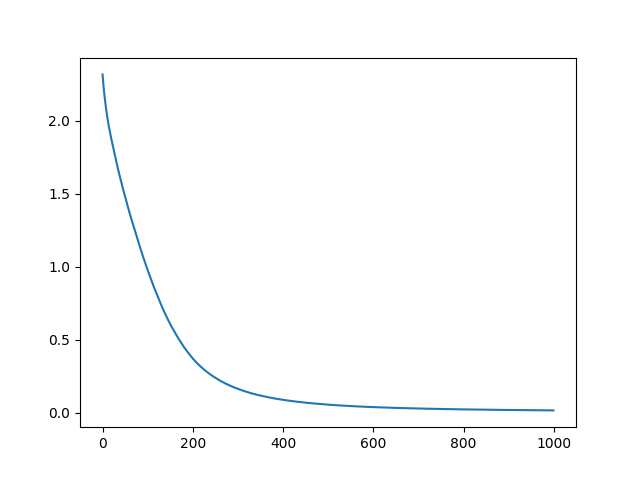
\includegraphics[width=\textwidth]{sanity_check.png}


The shape of the development of the loss function is almost exactly what we'd expect a nice satisfying 1/x curve. This suggests, since the derivative of this curve is logarithmic, that the rate of improvement decreases the more we have already learned, which makes sense. We also manage to get almost arbitrarily close to 0, suggesting that the network learns to recognize the training set perfectly, which allows us to conclude that the gradient computations are in fact working.

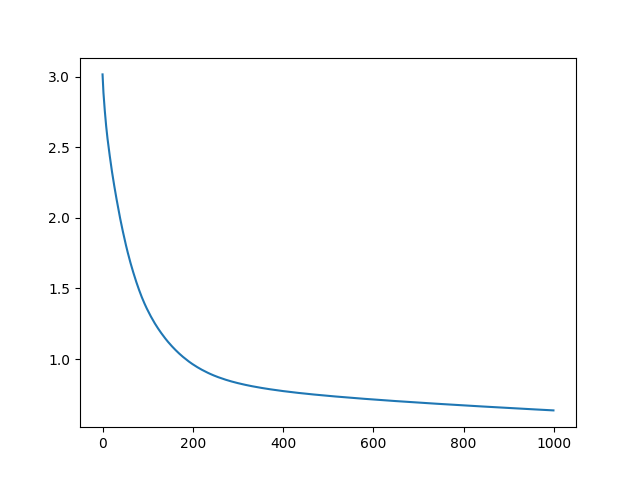
\includegraphics[width=\textwidth]{sanity_check_lambda-01.png}


When we set lambda to 0.01 we can see that we do not reach quite as low a value in our loss development, as expected, however we are still able to fit our net arbitrarily well.


\section{Training a k-layer network}

I began by training a 2 layer network with 1 hidden layer of 50 nodes. 
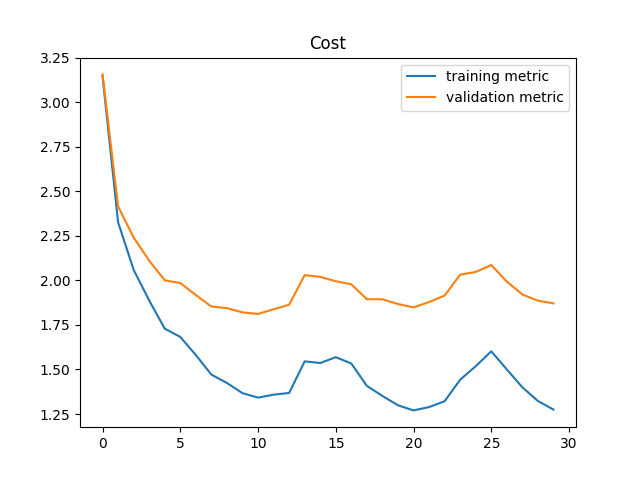
\includegraphics[width=\textwidth]{cost_k=1.png}
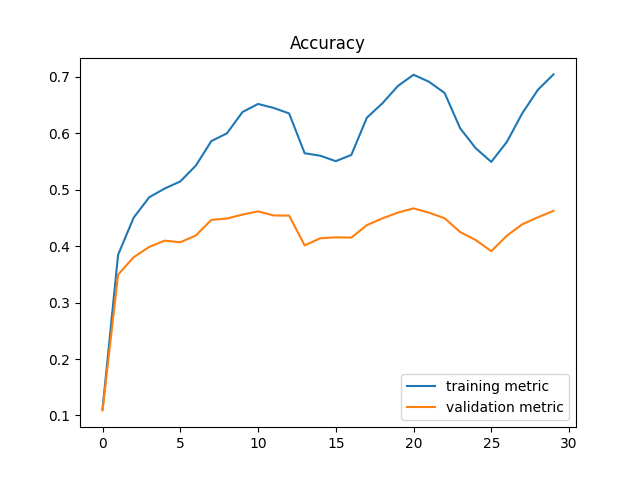
\includegraphics[width=\textwidth]{accuracy_k=1.png}\\

We can compare this with the results we got for a similar network from assignment 2\\
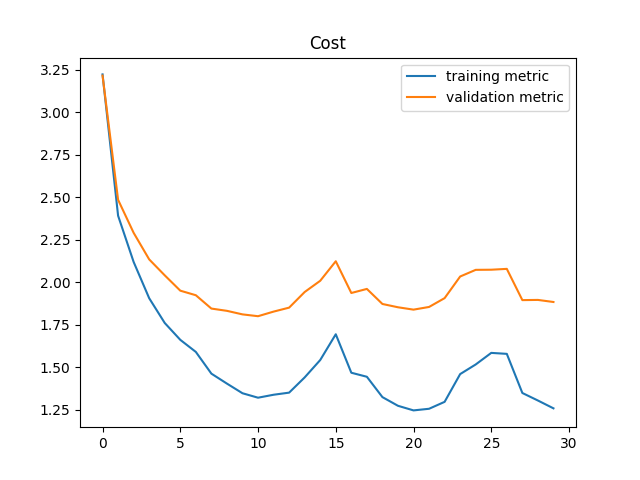
\includegraphics[width=\textwidth]{ns=800_cost.png}
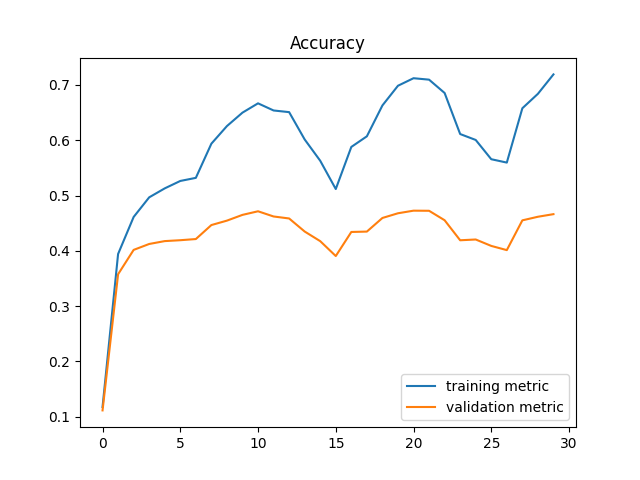
\includegraphics[width=\textwidth]{ns=800_accuracy.png}

The results look pretty similar.\\

If we add a second hidden layer also of 50 nodes, our metrics look as follows\\
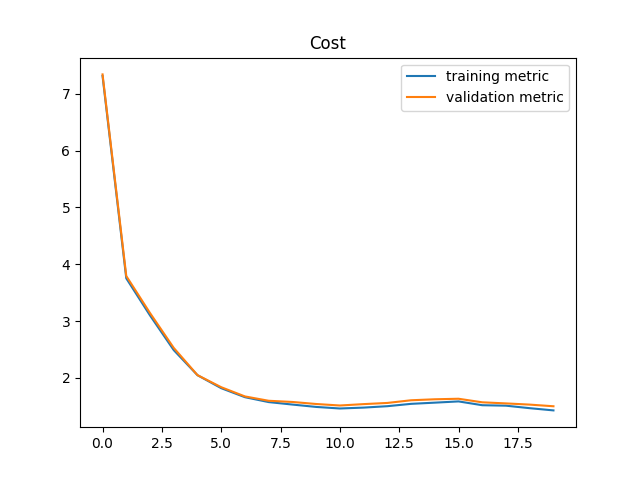
\includegraphics[width=\textwidth]{cost_k=2.png}
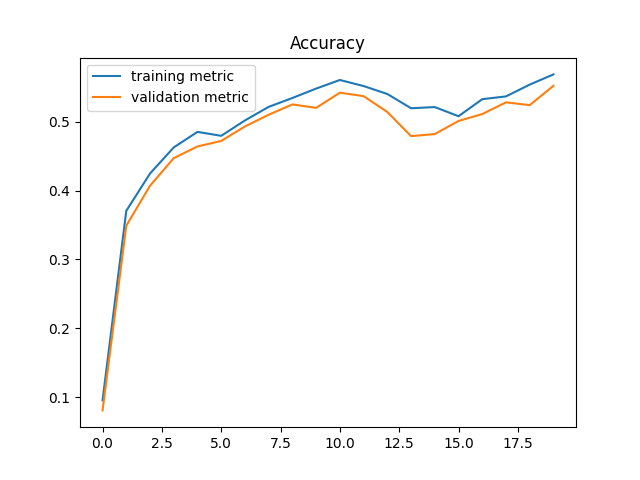
\includegraphics[width=\textwidth]{accuracy_k=2.png}
These graphs look pretty nice, the decrease in over fitting can be attributed to me switching to using the full training set.\\


The accuracy this 3 layer network exhibits on the test set is 0.5253333333333333. This test accuracy is however higher than my most performant network from assignment 2, suggesting that there's some value in increasing the depth of the network. If we investigate this assumption by attempting to train a 9 layer network, we see the following results\\


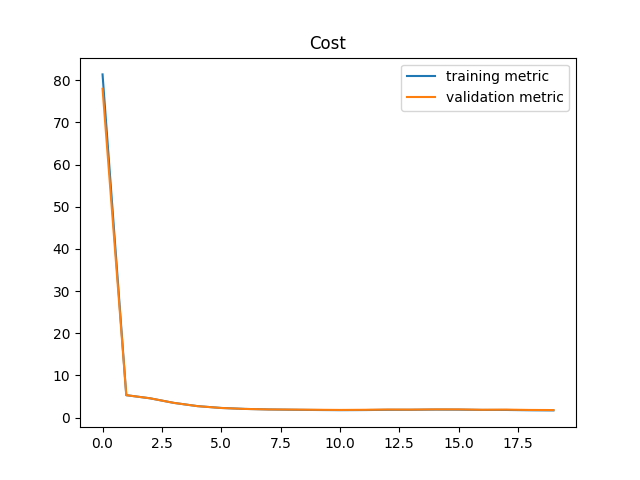
\includegraphics[width=\textwidth]{cost_k=9.png}
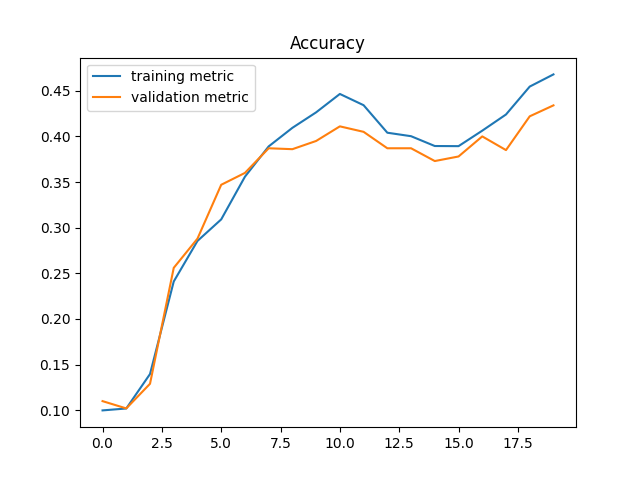
\includegraphics[width=\textwidth]{accuracy_k=9.png}

The test accuracy of this 9 layer network was 0.4488888888888889, almost an 8\% point decrease from our 3 layer network, no bueno.

\section{Implementing batch normalization}

I did not run into any troubles adapting my existing methods to include batch normalization. However, since I did not find instruction on how to initialize the gamma and beta parameters, I initialized beta's to 0, and gamma to 1's.\\

I performed the same sanity check as before, but on a network with batch normalization.

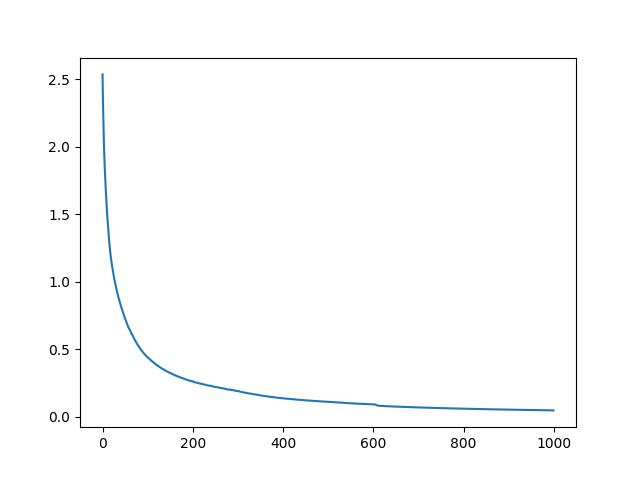
\includegraphics[width=\textwidth]{sanity_check_batch_norm.png}

We can see that the loss development looks the same as previously, suggesting that our gradient computations with batch normalization work well.

\section{Training a k-layer network with batch normalization}

We can re-attempt the previous training runs with batch normalization. Our 3 layer network with hidden layers = [50, 50] performs as follows:

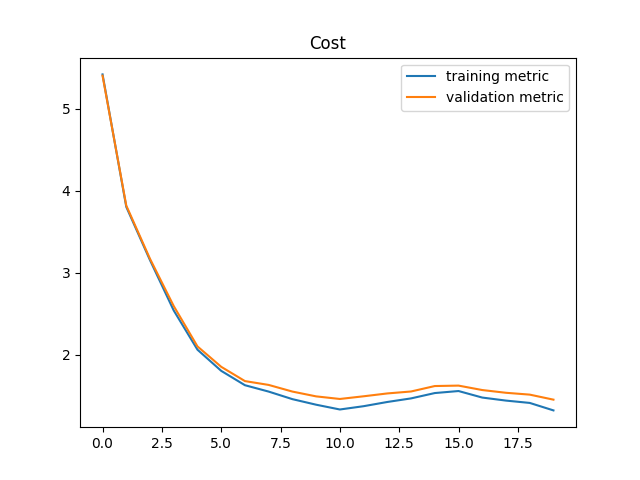
\includegraphics[width=\textwidth]{cost_k=2_batch_norm.png}
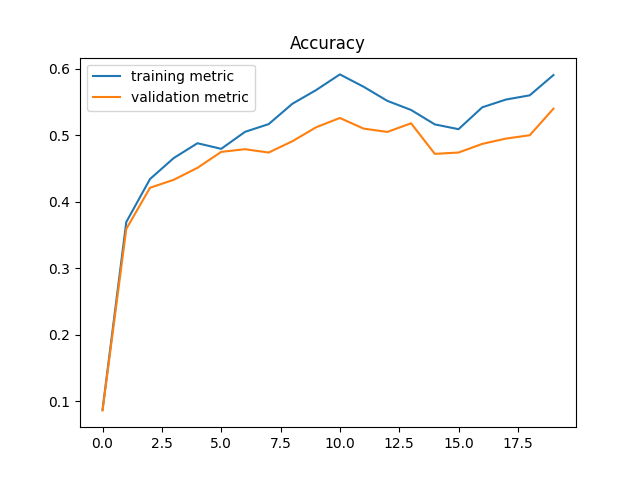
\includegraphics[width=\textwidth]{accuracy_k=2_batch_norm.png}

With a reported test accuracy of 0.5361111111111111. This seems to be a slight improvement to previously.

\subsection{Search for optimal lambda value}

I began by performing a coarse search with 10 uniformly sampled lambda values from the range 1E-1, 1E-5. The validation accuracy is plotted here.

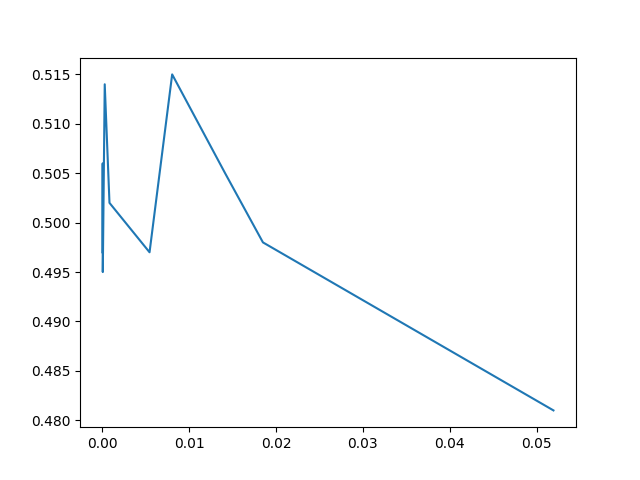
\includegraphics[width=\textwidth]{coarse_search.png}

As we can see the area of interest is roughly 0-0.015, with more emphasis to be placed on the upper end of this range.\\

Thus I performed a finer search by pulling 30 samples from a uniform distribution with domain [1E-4, 1E-2].\\

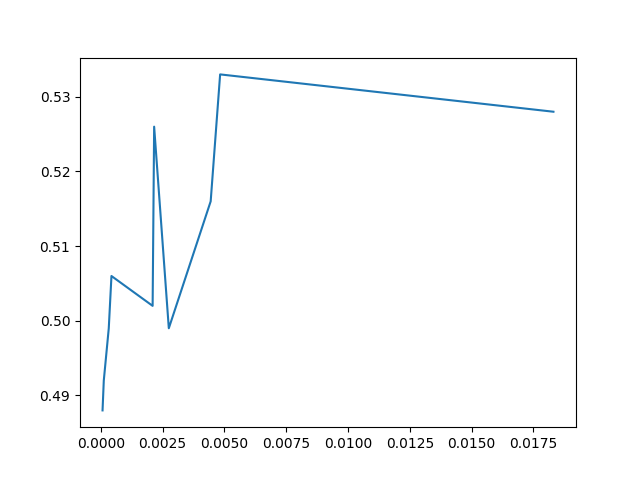
\includegraphics[width=\textwidth]{fine_search.png}



This fine search indicated that my optimal lambda setting would be ca. 0.0048. \\

The training metrics for my 3 layer network trained with this lambda are reported here:\\

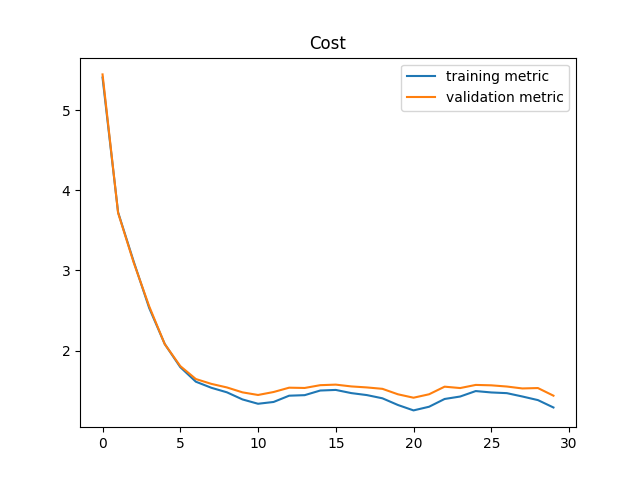
\includegraphics[width=\textwidth]{optimal_cost_k=3.png}
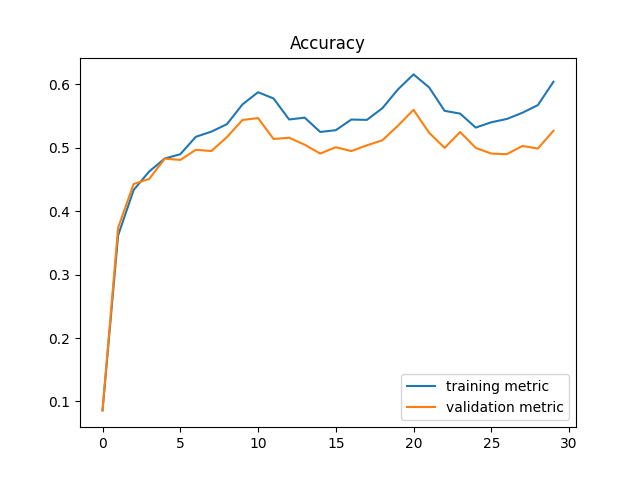
\includegraphics[width=\textwidth]{optimal_accuracy_k=3.png}

The test accuracy of this trained network is 0.54, the highest observed yet!\\

When training the 9 layer network of before with the same settings, this is what we see\\

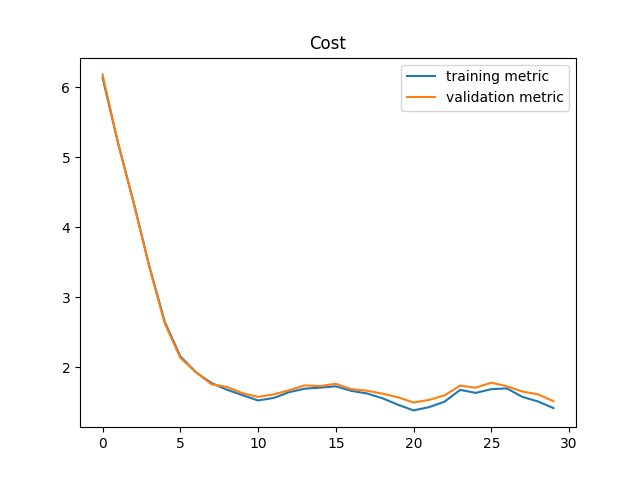
\includegraphics[width=\textwidth]{optimal_cost_k=9.png}
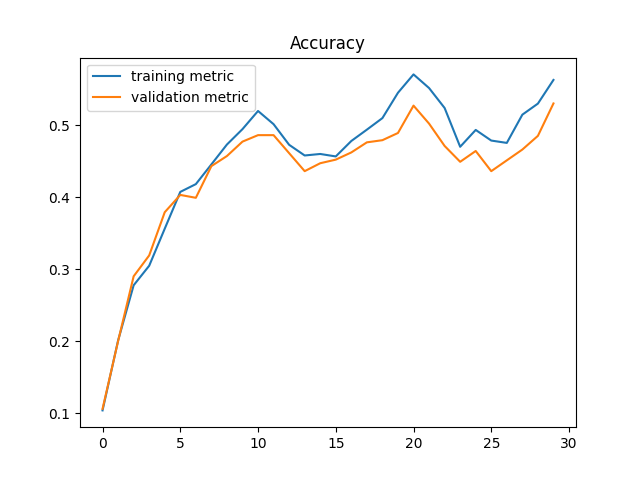
\includegraphics[width=\textwidth]{optimal_accuracy_k=9.png}

The reported test accuracy of this network is 0.5224444444444445, a substantial improvement.

\subsection{Batch normalization conclusion}

When comparing the graphs of the 3 layer networks with and without batch normalizaton, we can conclude that training with batch normalization seems to decrease over fitting, increase performance, and generally smoothen the training curves a bit. This suggests that training becomes more robust and regularized with batch normalization, even for the 3 layer networks.\\

When assessing the 9-layer network, the difference is night and day in performance numbers. We see more than a 15\% increase in test accuracy with batch normalization. This again confirms that training with batch normalization makes training more robust.

\section{Sensitivity to initialization}

\subsection{Batch norm}

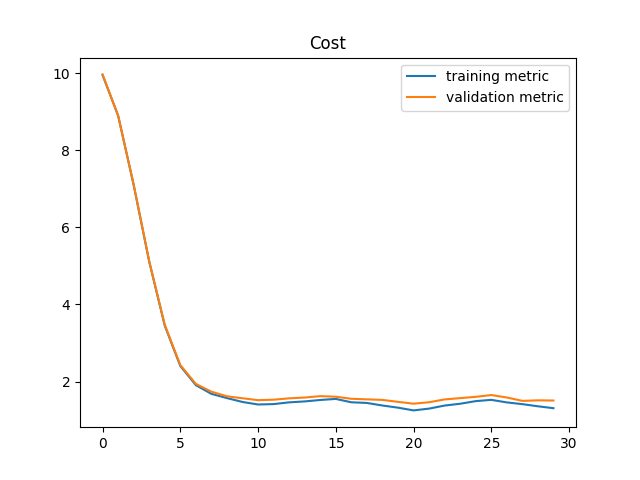
\includegraphics[width=\textwidth]{batch_norm_sig=1e-1_cost-.png}
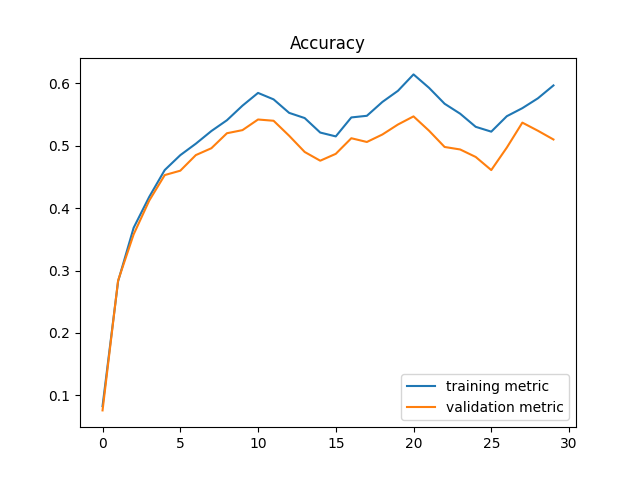
\includegraphics[width=\textwidth]{batch_norm_sig=1e-1_accuracy-.png}
Test accuracy sig 1e-1 acc = 0.5484444444444444\\


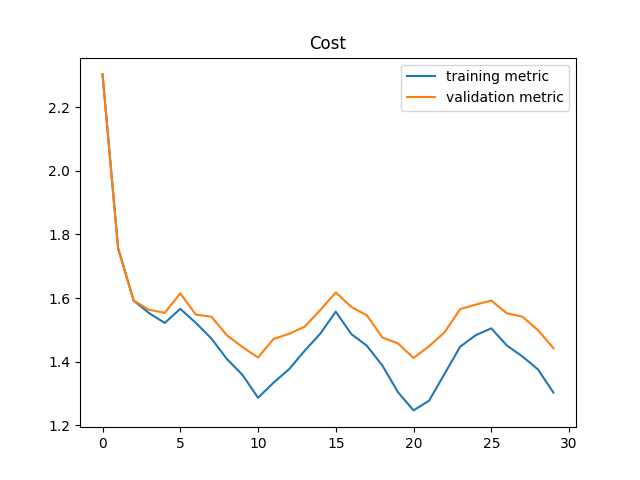
\includegraphics[width=\textwidth]{batch_norm_sig=1e-3_cost-.png}
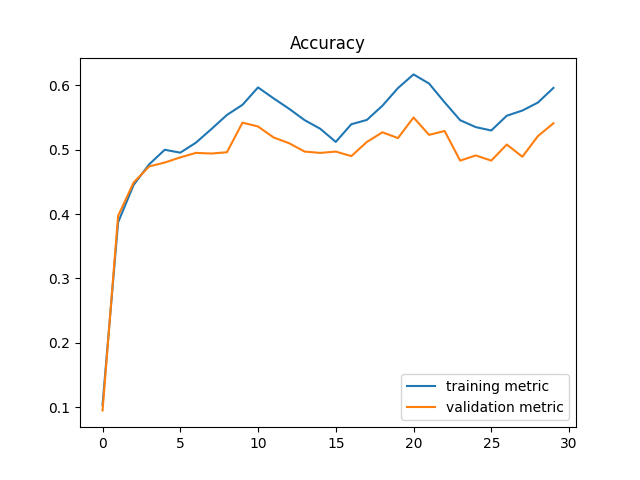
\includegraphics[width=\textwidth]{batch_norm_sig=1e-3_accuracy-.png}
Test accuracy sig 1e-3 acc = 0.5396666666666666\\


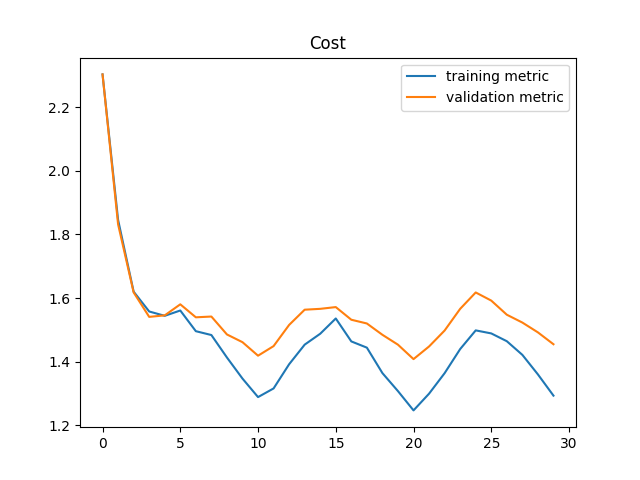
\includegraphics[width=\textwidth]{batch_norm_sig=1e-4_cost-.png}
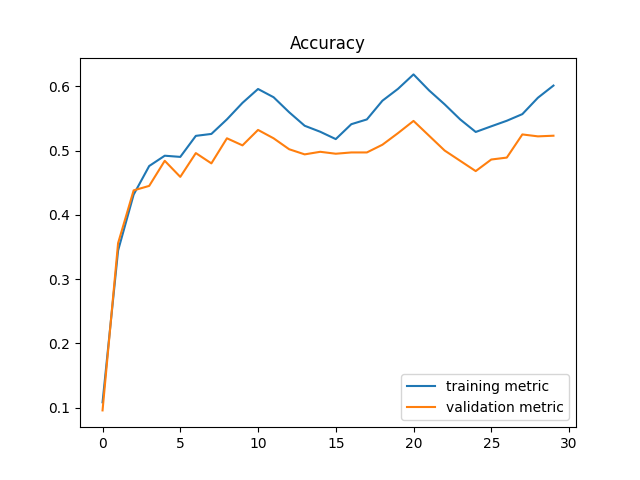
\includegraphics[width=\textwidth]{batch_norm_sig=1e-4_accuracy-.png}
Test accuracy sig 1e-4 acc = 0.5425555555555556\\

\subsection{Without batch norm}

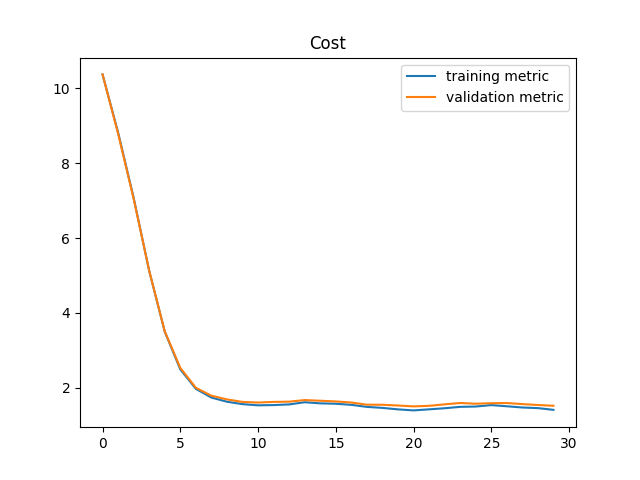
\includegraphics[width=\textwidth]{no_batch_norm_sig=1e-1_cost-.png}
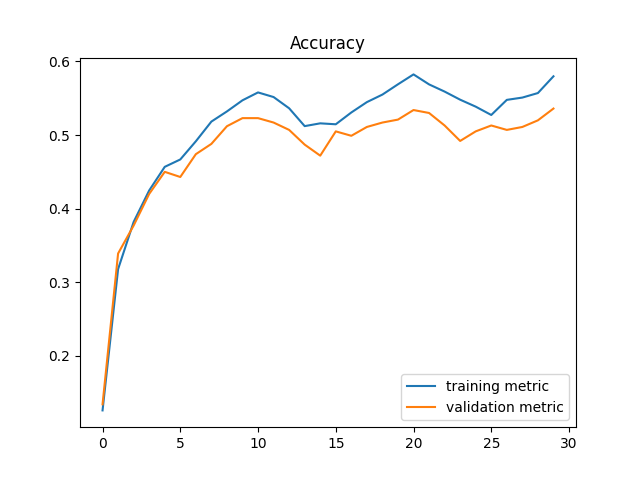
\includegraphics[width=\textwidth]{no_batch_norm_sig=1e-1_accuracy-.png}
Sig 1e-1 acc = 0.5341111111111111\\
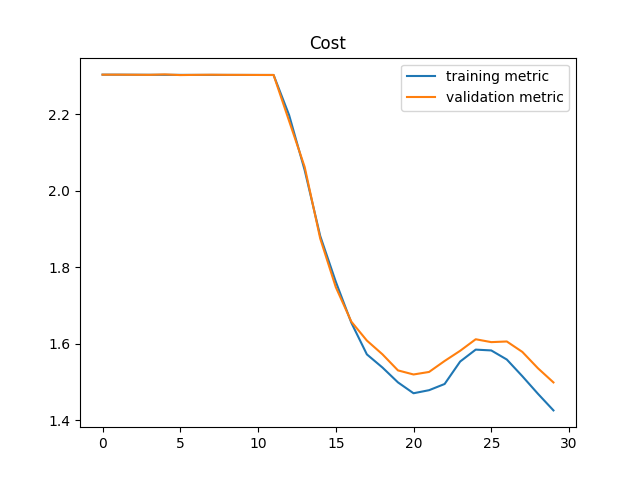
\includegraphics[width=\textwidth]{no_batch_norm_sig=1e-3_cost-.png}
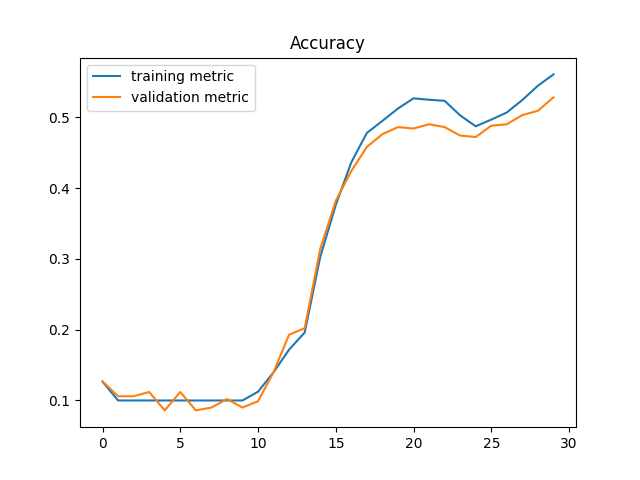
\includegraphics[width=\textwidth]{no_batch_norm_sig=1e-3_accuracy-.png}
Sig 1e-3 acc = 0.5271111111111111\\
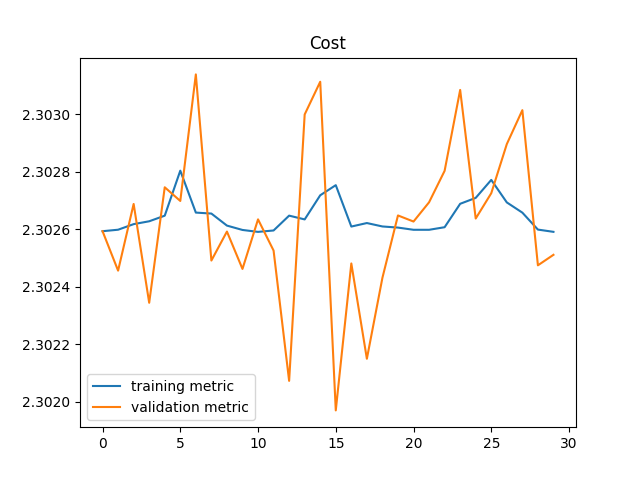
\includegraphics[width=\textwidth]{no_batch_norm_sig=1e-4_cost-.png}
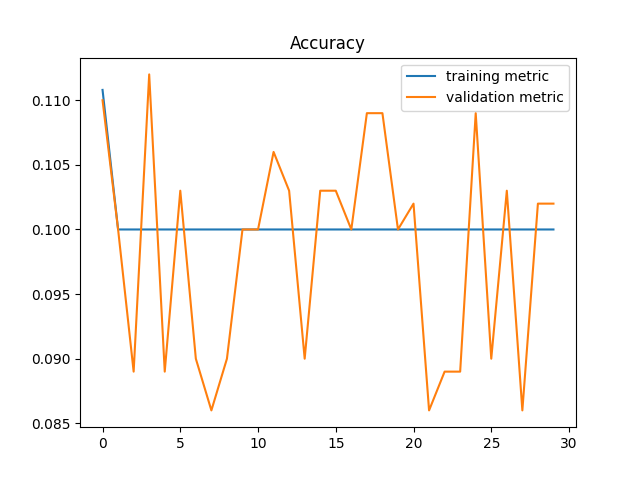
\includegraphics[width=\textwidth]{no_batch_norm_sig=1e-4_accuracy-.png}
Sig 1e-4 acc = 0.09977777777777778


As we can see here, training the network with batch normalization leads to a much more stable training loop for smaller standard deviations when initializing the network parameters. This suggests that batch normalization makes training more robust to initialization.
\end{document}
